\section{Suggested Model}
\label{sec:model}

Finally, we exploit {\mlr} to generate regression model for three responses \texttt{casual,registered,cnt}. The results are shown as follows.

\subsection{Cnt}
\begin{lstlisting}[style=rlanguage]
Call:
lm(formula = cnt ~ season + yr + mnth + hr + holiday + weekday +
    weathersit + (temp + hum + windspeed)^2 + poly(hum, 4) +
    I(windspeed^2), data = bicycle)

Residuals:
    Min      1Q  Median      3Q     Max
-366.40  -59.41   -5.70   50.19  424.33

Coefficients: (1 not defined because of singularities)
               Estimate Std. Error t value Pr(>|t|)
(Intercept)    -150.337     13.187 -11.400  < 2e-16 ***
seasonSpring    -31.664      5.699  -5.556 2.80e-08 ***
seasonSummer      8.979      4.925   1.823  0.06831 .
seasonWinter     35.209      5.115   6.883 6.06e-12 ***
yry1             84.671      1.559  54.324  < 2e-16 ***
...
weathersitMist   -9.529      1.909  -4.992 6.02e-07 ***
weathersitRain  -83.097     58.292  -1.426  0.15403
weathersitSnow  -60.884      3.387 -17.976  < 2e-16 ***
temp            380.473     19.070  19.951  < 2e-16 ***
hum             114.093     14.960   7.626 2.54e-14 ***
windspeed        85.546     36.478   2.345  0.01903 *
poly(hum, 4)1        NA         NA      NA       NA
poly(hum, 4)2  -989.456    113.454  -8.721  < 2e-16 ***
poly(hum, 4)3   289.732    103.030   2.812  0.00493 **
poly(hum, 4)4   274.210    104.049   2.635  0.00841 **
I(windspeed^2) -215.503     36.334  -5.931 3.07e-09 ***
temp:hum       -340.669     24.058 -14.161  < 2e-16 ***
temp:windspeed  190.288     35.142   5.415 6.21e-08 ***
hum:windspeed  -181.499     35.112  -5.169 2.38e-07 ***
---
Signif. codes:  0 ‘***’ 0.001 ‘**’ 0.01 ‘*’ 0.05 ‘.’ 0.1 ‘ ’ 1

Residual standard error: 100.6 on 17320 degrees of freedom
Multiple R-squared:  0.6933,	Adjusted R-squared:  0.6923
F-statistic: 675.1 on 58 and 17320 DF,  p-value: < 2.2e-16
\end{lstlisting}

\subsection{Casual}
\begin{lstlisting}[style = rlanguage]
> lm.fit_fin = lm(casual~season+yr+mnth+hr+holiday+weekday+weathersit+(temp+hum+windspeed)^2+poly(hum,4)+I(windspeed^2),data=bicycle)
> summary(lm.fit_fin)

Call:
lm(formula = casual ~ season + yr + mnth + hr + holiday + weekday +
    weathersit + (temp + hum + windspeed)^2 + poly(hum, 4) +
    I(windspeed^2), data = bicycle)

Residuals:
    Min      1Q  Median      3Q     Max
-91.485 -18.393  -3.001  12.852 251.042

Coefficients: (1 not defined because of singularities)
                Estimate Std. Error t value Pr(>|t|)
(Intercept)     -36.9387     4.0705  -9.075  < 2e-16 ***
seasonSpring     -1.5635     1.7591  -0.889 0.374127
seasonSummer      9.0139     1.5203   5.929 3.10e-09 ***
seasonWinter      0.4354     1.5790   0.276 0.782745
yry1             11.6976     0.4811  24.314  < 2e-16 ***
...
temp            158.5548     5.8865  26.935  < 2e-16 ***
hum              50.0185     4.6179  10.831  < 2e-16 ***
windspeed        -5.3359    11.2598  -0.474 0.635584
poly(hum, 4)1         NA         NA      NA       NA
poly(hum, 4)2  -218.2046    35.0205  -6.231 4.75e-10 ***
poly(hum, 4)3    82.0113    31.8030   2.579 0.009925 **
poly(hum, 4)4   101.5730    32.1174   3.163 0.001567 **
I(windspeed^2)  -53.8757    11.2155  -4.804 1.57e-06 ***
temp:hum       -152.3517     7.4260 -20.516  < 2e-16 ***
temp:windspeed   72.3110    10.8474   6.666 2.70e-11 ***
hum:windspeed   -31.4267    10.8382  -2.900 0.003741 **
---
Signif. codes:  0 ‘***’ 0.001 ‘**’ 0.01 ‘*’ 0.05 ‘.’ 0.1 ‘ ’ 1

Residual standard error: 31.06 on 17320 degrees of freedom
Multiple R-squared:  0.6045,	Adjusted R-squared:  0.6032
F-statistic: 456.5 on 58 and 17320 DF,  p-value: < 2.2e-16
\end{lstlisting}

\subsection{Registered}
\begin{lstlisting}[style=rlanguage]
> lm.fit_fin = lm(registered~season+yr+mnth+hr+holiday+weekday+weathersit+(temp+hum+windspeed)^2+poly(hum,4)+I(windspeed^2),data=bicycle)
> summary(lm.fit_fin)

Call:
lm(formula = registered ~ season + yr + mnth + hr + holiday +
    weekday + weathersit + (temp + hum + windspeed)^2 + poly(hum,
    4) + I(windspeed^2), data = bicycle)

Residuals:
    Min      1Q  Median      3Q     Max
-346.74  -48.33   -4.84   45.05  409.22

Coefficients: (1 not defined because of singularities)
                 Estimate Std. Error t value Pr(>|t|)
(Intercept)    -113.39857   11.12982 -10.189  < 2e-16 ***
seasonSpring    -30.10083    4.80975  -6.258 3.98e-10 ***
seasonSummer     -0.03502    4.15677  -0.008 0.993279
seasonWinter     34.77392    4.31732   8.055 8.49e-16 ***
yry1             72.97351    1.31547  55.473  < 2e-16 ***
...
I(windspeed^2) -161.62695   30.66584  -5.271 1.38e-07 ***
temp:hum       -188.31749   20.30450  -9.275  < 2e-16 ***
temp:windspeed  117.97659   29.65931   3.978 6.99e-05 ***
hum:windspeed  -150.07255   29.63427  -5.064 4.14e-07 ***
---
Signif. codes:  0 ‘***’ 0.001 ‘**’ 0.01 ‘*’ 0.05 ‘.’ 0.1 ‘ ’ 1

Residual standard error: 84.92 on 17320 degrees of freedom
Multiple R-squared:  0.6863,	Adjusted R-squared:  0.6852
F-statistic: 653.2 on 58 and 17320 DF,  p-value: < 2.2e-16
\end{lstlisting}

\subsection{Graphs}
Here we present the residual graph for all the three predictors. From the following three graphs we could observe that there are no explicit patterns in \texttt{Residual vs Fitted} graph, indicating that a linear model could describe the relationship between predictors and response well. Moreover, most points in \texttt{Normal Q-Q} graph locates near the line with the slope of 45 degree thus the standardized residuals obeys to a normal distribution with $\sigma = 0$, which means that the normality hypothesis holds.

\begin{figure}[ht]
  \centering
  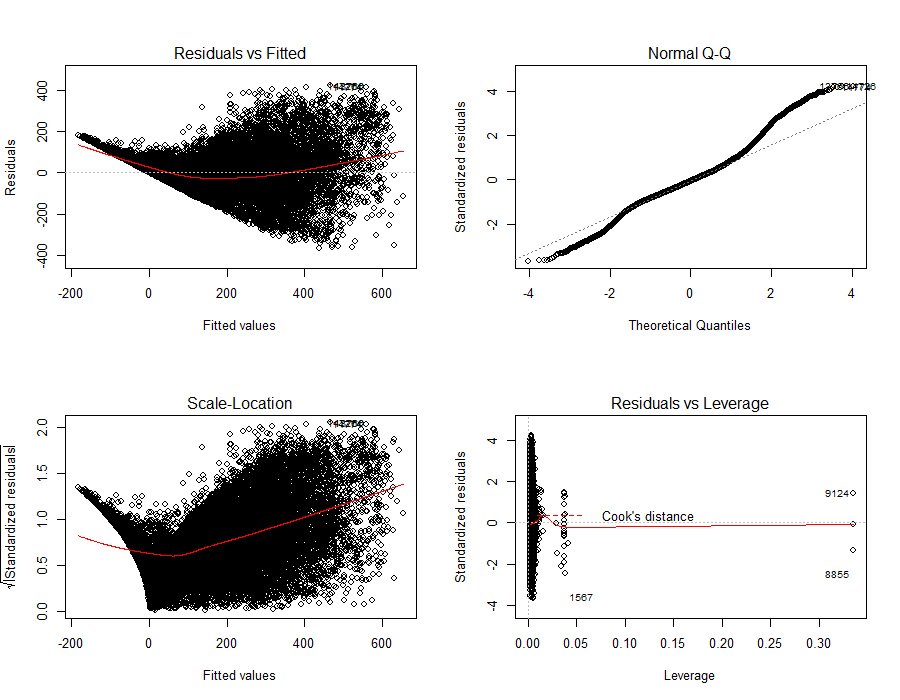
\includegraphics[width=\linewidth]{pic/cnt.png}\\
  \caption{Residual Graphs about Response \texttt{cnt}}\label{fig:cnt}
\end{figure}

\begin{figure}[ht]
  \centering
  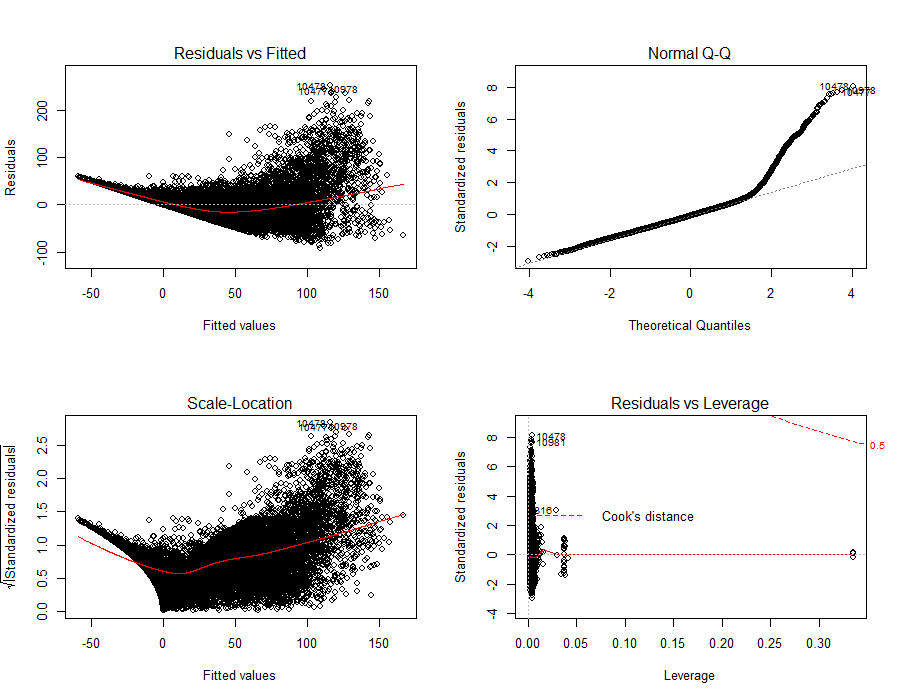
\includegraphics[width=\linewidth]{pic/casual.png}\\
  \caption{Residual Graphs about Response \texttt{casual}}\label{fig:casual}
\end{figure}

\begin{figure}[ht]
  \centering
  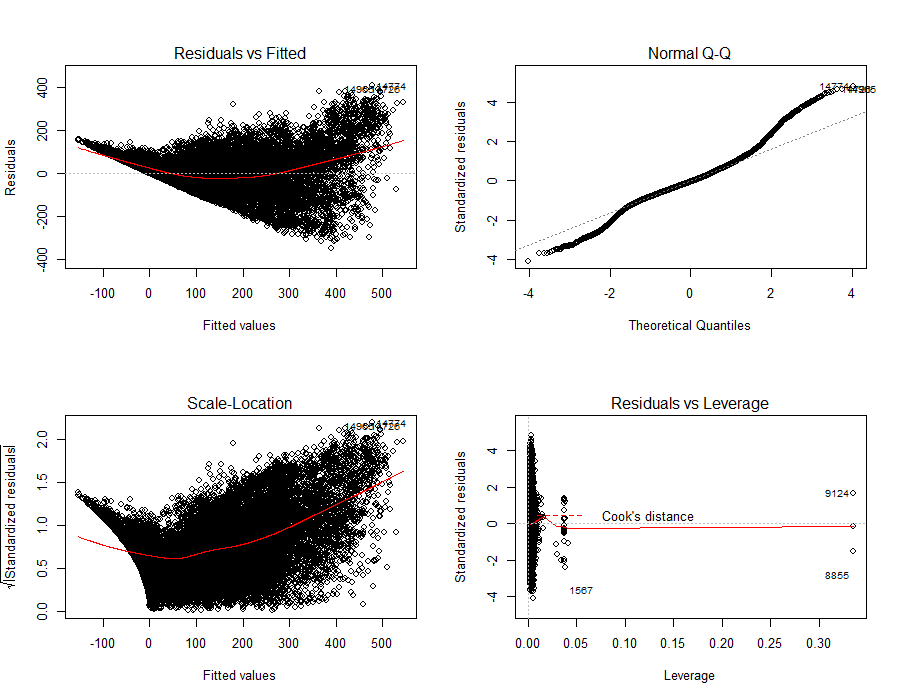
\includegraphics[width=\linewidth]{pic/registered.png}\\
  \caption{Residual Graphs about Response \texttt{registered}}\label{fig:registered}
\end{figure}

\subsection{Questions}
Now we could answer the seven important questions.
\begin{enumerate}
  \item \textit{Is there a relationship between predictors and responses?}\\
   We first set the null hypothesis, $H_0 = \beta_0 = \beta_1 = ... = \beta_p = 0$. Then we compute the F-statistic, which tells us if we should reject the null hypothesis:
      \\$F-statistic$ = 456.5 on 58 and 17320 DF  \\$p-value <$ 2.2e-16\\
   A high F-statistic and low p-value indicate clear evidence between predictors and responses.

  \item \textit{How strong is the relationship between predictors and responses?}\\
      We compute two measures: RSE and $R^2$.\\
       RSE (Residual Standard Error): standard deviation of the response from the population regression line;
       \begin{equation}\label{equ:rse}
         RSE = \sqrt{\frac{1}{n-p-1}RSS}
       \end{equation}
        $R^2$: percentage of variability in the response that is explained by the predictors.
        \begin{equation}\label{equ:rsq}
        R^2 = \frac{TSS-RSS}{TSS} = 1-\frac{RSS}{TSS}
       \end{equation}
       Taking \texttt{registered} as an example, RSE = 84.92 and $R^2$ = 0.6852, thus almost 70\% of variance in \texttt{registered} is explained by the predictors.
  \item \textit{Which predictors contribute to responses?}\\
      From the summary  in Section~\ref{sec:fitall} we could find that after data transformation, all predictors except \texttt{atemp} and \texttt{workingday} contribute to the responses.
  \item \textit{ How accurately can we estimate the effect of each predictor on responses?}\\
      We can use \texttt{confint} function to construct 95\% confidence intervals $(2 \times SE(\hat{\beta_i})$ for each $X_i$).
      \begin{lstlisting}[style=rlanguage]
> confint(lm.fit_reg)
                       2.5 %        97.5 %
(Intercept)    -135.21414187  -91.58299531
seasonSpring    -39.52842681  -20.67323457
seasonSummer     -8.18271186    8.11267767
seasonWinter     26.31153938   43.23629561
...
poly(hum, 4)4     0.50778077  344.76708025
I(windspeed^2) -221.73508938 -101.51881134
temp:hum       -228.11636613 -148.51860843
temp:windspeed   59.84134008  176.11184295
hum:windspeed  -208.15871196  -91.98639067
\end{lstlisting}
  \item \textit{How accurately can we predict future responses?}\\
      To predict an \emph{individual response}, $Y = f(X) + \epsilon$, we can calculate prediction interval.
\begin{lstlisting}[style = rlanguage]
>predict(lm.fit_reg,data.frame(season="Spring",yr = "y0",mnth ="m2", holiday = "No", hr = "h10",weekday = "w5", weathersit="Clear",temp = 0.24, atemp = 0.2879,hum=0.80,windspeed = 0.2),interval="prediction")
      fit       lwr      upr
1 40.1079 -126.6063 206.8221
\end{lstlisting}
Thus 95\% \textbf{Prediction Interval} is [-126.6063, 206.8221].\\
To predict an \emph{average response}, $f(X)$, we can calculate confidence interval.
\begin{lstlisting}[style = rlanguage]
> predict(lm.fit_reg,data.frame(season="Spring",yr = "y0",mnth ="m2", holiday = "No", hr = "h10",weekday = "w5", weathersit="Clear",temp = 0.24, atemp = 0.2879,hum=0.80,windspeed = 0.2),interval="confidence")
      fit      lwr      upr
1 40.1079 30.76016 49.45563
\end{lstlisting}
Thus 95\% \textbf{Confidence Interval} is [30.76016, 49.45563].
  \item \textit{Is the relationship linear?}\\
  Not all predictors are linear according to our analysis in Section~\ref{sec:non-linear}, therefore we transform some predictors to accommodate non-linear relationships.
  \item \textit{ Is there synergy among the predictors?}\\
  Based on the analysis in Section~\ref{sec:interactive}, between many pairs of predictors there are strong interactions such as \texttt{temp:hum} with $p-value < 2e-16$.
      
\end{enumerate}
